\documentclass[12pt,twoside, letter]{exam}
\usepackage{enumitem, kantlipsum}
\usepackage[margin=1in,left=1in,right=1in,top=1in,bottom=1in]{geometry}
\usepackage{graphicx,epstopdf}
\usepackage{amssymb,amsmath,amsfonts, amsthm}
\usepackage{wasysym}
\newtheorem{theorem}{Theorem}
\newtheorem{corollary}{Corollary}[theorem]
\newtheorem{lemma}[theorem]{Lemma}
\usepackage{hyperref}
\usepackage{tikz}
\usepackage{xstring}
\usetikzlibrary{calc}
\usepackage{ducksay}
\newtheorem{prop}{Proposition}

\theoremstyle{definition}
\newtheorem{definition}{Definition}

\usepackage{bbm}
\usepackage{verbatim}
\usepackage{bbold}
\usepackage{phfparen}
\usepackage{sets}
\newcommand{\nn}{\mathbb{N}}
\newcommand{\rr}{\mathbb{R}}
\newcommand{\cc}{\mathbb{C}}
\newcommand{\cb}{\mathcal{B}}
\newcommand{\ctau}{\mathcal{T}}
\newcommand{\co}{\mathcal{O}}
\newcommand{\zz}{\mathbb{Z}}
\newcommand{\ee}{\mathbb{E}}
\newcommand{\qq}{\mathbb{Q}}
\newcommand{\interior}{\text{Int}}
\newcommand{\pp}{\mathbb{P}}
\newcommand{\id}{\mathbbm{1}}
\newcommand{\Co}{\text{Co}}
\newcommand{\Cl}{\text{Cl}}
\usepackage{mathtools}
\DeclarePairedDelimiter\ceil{\lceil}{\rceil}
\DeclarePairedDelimiter\floor{\lfloor}{\rfloor}


\usepackage{indentfirst}
\setlist{
    listparindent = \parindent,
    parsep = 6pt,
}

\makeatletter
\newsavebox\myboxA
\newsavebox\myboxB
\newlength\mylenA

\newcommand*\xoverline[2][0.9]{%
    \sbox{\myboxA}{$\m@th#2$}%
    \setbox\myboxB\null% Phantom box
    \ht\myboxB=\ht\myboxA%
    \dp\myboxB=\dp\myboxA%
    \wd\myboxB=#1\wd\myboxA% Scale phantom
    \sbox\myboxB{$\m@th\overline{\copy\myboxB}$}%  Overlined phantom
    \setlength\mylenA{\the\wd\myboxA}%   calc width diff
    \addtolength\mylenA{-\the\wd\myboxB}%
    \ifdim\wd\myboxB<\wd\myboxA%
       \rlap{\hskip 0.5\mylenA\usebox\myboxB}{\usebox\myboxA}%
    \else
        \hskip -0.5\mylenA\rlap{\usebox\myboxA}{\hskip 0.5\mylenA\usebox\myboxB}%
    \fi}
\makeatother

\usepackage{float}
\floatstyle{boxed}
\restylefloat{figure}

\printanswers

\begin{document}


\abovedisplayskip=12pt
\belowdisplayskip=12pt
\abovedisplayshortskip=7pt
\belowdisplayshortskip=10pt
\allowdisplaybreaks

\setlength{\parindent}{18pt}

\title{Quantitative Methods: Assignment 4}
\author{Raymond Luo}
\date{\today}
\maketitle

\noindent {\bf Problem 1 (35 points):}
  \begin{enumerate}
    \item Write a code in Matlab to simulate a Poisson process $N(t)$ with parameter $\lambda > 0$ over the
      time interval $[0,T]$ where $T > 0$.
      \begin{solution}
        \begin{figure}[H]
          \centering
            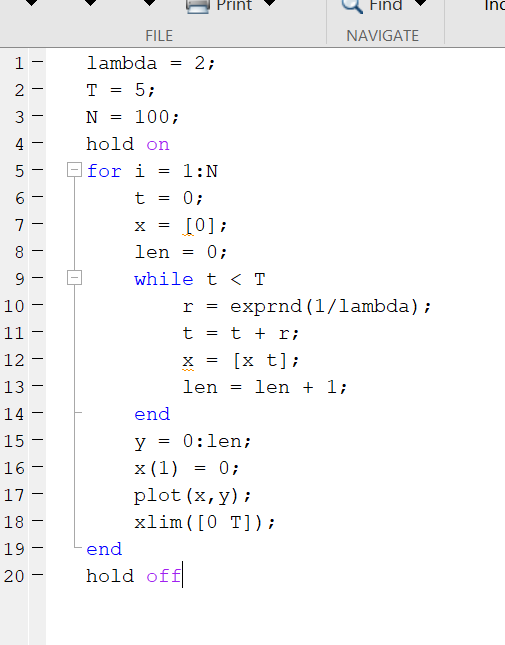
\includegraphics[width=3in]{Hw4_1a}
        \end{figure}
      \end{solution}
    \item Take $T = 5$ year, $\lambda = 2$ per year. Plot 100 sample paths.
      \begin{solution}
        \begin{figure}[H]
          \centering
            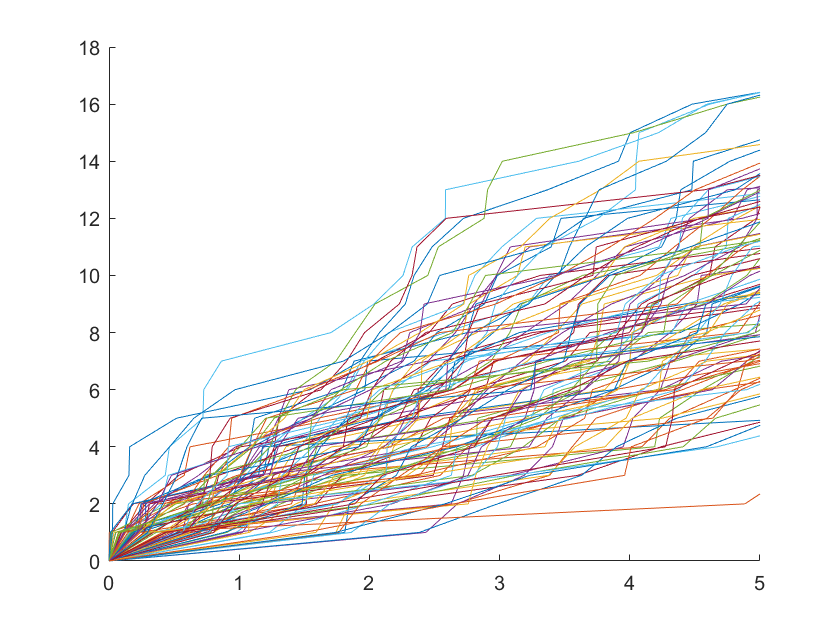
\includegraphics[width=3in]{Hw4_1}
        \end{figure}
      \end{solution}
  \end{enumerate}



\noindent {\bf Problem 2 (25 points):}
\par{ Consider the following process $\{X(t), t\geq 0\}$ defined by}
  \begin{equation*}
    X(t) = N(t) - \lambda t
  \end{equation*}
where $N$ is a Poisson process with rate $\lambda > 0$
  \begin{enumerate}
    \item What is the probability mass of $X(t)$?
      \begin{solution}
        We note that $N(t) = N(t) - 0 = N(t) - N(0) \sim Pois(\lambda t)$. It then follows that the pmf of $X(t)$ is
        $\pp[X(t) = n] = \pp[N(t) - \lambda t = n] = \pp[N(t) = n + \lambda t]$. We can then intuitively observe that
        this is a Poisson process that has mean zero at each arrival time. \\
        Alternatively, we can describe the process by its increments after observing that $X(0) = N(0) - 0 = 0$:
        $\forall t,s \geq 0, X(s+t) - X(t) = N(s+t) - \lambda(s+t) - N(t) + \lambda(t) = N(s+t) - N(t) - \lambda s$.
        As $N(s+t) - N(t) \sim Pois(\lambda s)$, we observe that each increment of our process follows the probability
        distribution of a Poisson distribution with parameter $\lambda s$ but re-centered to have mean 0 through translation. 
      \end{solution}
    \item Give the expectation and the variance of $X(t)$.
      \begin{solution}
        The expectation is $\ee[X(t)] = \ee[N(t) - \lambda t] = \ee[N(t)] - \lambda t = \lambda t - \lambda t = 0 $\\
        The variance is $Var[X(t)] = Var[N(t) - \lambda t] = Var[N(t)] = \lambda t$
      \end{solution}
    \item Is $X$ a martingale? Justify your answer
      \begin{solution}
        $X$ is a martingale as $\ee[X(t+s) \mid X(t)] = \ee[X(t+s) - X(t) + X(t) \mid X(t)]
        = \ee[X(t+s) - X(t) \mid X(t)] + \ee[X(t)\mid X(t)] = \ee[N(t+s) - \lambda (t+s) - N(s) + \lambda (s) \mid X(t)] + X(t)
        = \ee[N(t+s) - N(s) - \lambda s \mid X(t)] + X(t) = \lambda s - \lambda s + X(t) = X(t)$
      \end{solution}
  \end{enumerate}

\noindent {\bf Problem 3 (40 points):} We model the aggregate insurance loss, at time $t$, as follows:
  \begin{equation*}
    S(t) = S(0) + \sum^{N(t)}_{i=1} X_{i},
  \end{equation*}
  where $S(0)$ is a given real number, $X_{i}$ are independent exponential variables with rate $\mu$, and
  $\{N(t), t \geq 0\}$ is a Poisson process with rate $\lambda$, independent of $X_{i}$. When $N(t) = 0$, we simply
  set $\sum^{N(t)}_{i=0} X_{i} = 0$. The common mean of the exponential variables is $\frac{1}{\mu}$ and their variance is $\frac{1}{\mu^2}$.

  \begin{enumerate}
    \item Compute $\ee[S(t)]$
      \begin{solution}
        $\ee[S(t)] = \ee[S(0) + \sum^{N(t)}_{i=1} X_{i}] = S(0) + \ee[\ee[\sum^{N(t)}_{i=1} X_{i} \mid N(t)]] \\
        = S(0) + \sum^\infty_{n = 0} \ee[\sum^{N(t)}_{i=1} X_{i} \mid N(t) = n]\cdot\pp[N(t) = n] \\
        = S(0) + \sum^{\infty}_{n=0} n\ee[X_{1}] \cdot \pp[N(t) = n] = S(0) + \ee[N(t)\cdot \ee[X_{1}]]
        = S(0) + \ee[\frac{N(t)}{\mu}] = S(0) + \frac{1}{\mu}\cdot(\lambda t) = S(0) + \frac{\lambda t}{\mu}$
      \end{solution}
    \item Compute $\ee[S^{2}(t)]$
      \begin{solution}
        $\ee[S^{2}(t)] = \ee[S^2(0) + 2\sum^{N(t)}_{i=1} X_{i} S(0) + \sum^{N(t)}_{i=1}\sum^{N(t)}_{j = 1} X_{i}X_{j}] \\
        = S^{2}(0) + 2 \cdot S(0)\cdot \ee[\sum^{N(t)}_{i=1} X_{i}] + \ee[\sum^{N(t)}_{i=1}\sum^{N(t)}_{j = 1} X_{i}X_{j}] \\
        = S^2(0) + 2 \cdot S(0)\frac{\lambda t}{\mu} + \ee[\sum^{N(t)}_{i=1}\sum^{N(t)}_{j = 1} X_{i}X_{j}] \\
        \text{ [by using substitution from steps in previous problem]} \\
        = S^2(0) + S(0)\frac{2\lambda t}{\mu} + \ee[\ee[\sum^{N(t)}_{i=1}\sum^{N(t)}_{j = 1} X_{i}X_{j}] \mid N(t)] $\\
        We then focus on the last term: \\
        $\sum^{\infty}_{n = 0}\ee[\sum^{n}_{i=1}\sum^{n}_{j = 1} X_{i}X_{j}] \pp(N(t) = n) \\
        = \sum^{\infty}_{n = 0} \big(\sum_{i\neq j} \ee[X_{i}X_{j}] + \sum^{n}_{i = 1} \ee[X_{i}^2] \big) \pp(N(t) = n) \\
        = \sum^{\infty}_{n = 0} \big(\frac{n^2-n}{\mu^{2}} + \sum^{n}_{i = 1} (Var[X_i] + \ee[X_i]^2) \big) \pp(N(t) = n) \\
        = \sum^{\infty}_{n = 0} \big(\frac{n^2-n}{\mu^{2}} + \sum^{n}_{i = 1} \frac{2}{\mu^2} \big) \pp(N(t) = n) \\
        = \sum^{\infty}_{n = 0} \frac{n^2 + n}{\mu^{2}} \pp(N(t) = n) \\
        = \frac{1}{\mu^{2}} \sum^{\infty}_{n = 0} \big(n^2 \cdot \pp(N(t)) + n \cdot \pp(N(t)) \big)\\
        = \frac{1}{\mu^{2}}\big(\ee[N(t)] + \ee[N(t)^2] \big) \\
        = \frac{1}{\mu^{2}}\big(\ee[N(t)] + Var[N(t)] + \ee[N(t)]^2 \big) \\
        = \frac{1}{\mu^{2}}\big(\lambda t + \lambda t + \lambda^2 t^2 \big) = \frac{\lambda^2 t^2 + 2\lambda t}{\mu^2}$ \\
        Thus we have: \\
        $\ee[S^{2}(t)] = S^2(0) + S(0) \frac{2\lambda t}{\mu} + \frac{\lambda^2 t^2 + 2\lambda t}{\mu^2}$
      \end{solution}
  \end{enumerate}

\end{document}
